\chapterdivider{8}{Visualization: parameter space and state space}
  {Which plot answers the scientific question in front of me?}
  {Featured application: FitzHugh--Nagumo before and after a Hopf transition}

\begin{frame}{One model, three complementary views}
\small
\begin{center}
\begin{tabular}{>{\raggedright\arraybackslash}p{.25\textwidth}
                >{\raggedright\arraybackslash}p{.30\textwidth}
                >{\raggedright\arraybackslash}p{.34\textwidth}}
\toprule
View & Question answered & What it does not establish\\
\midrule
Bifurcation diagram & How equilibria or cycles change with $p$ & Flow geometry or basins at one fixed $p$\\
Eigenvalue/Floquet plot & How local stability changes & Nonlinear trajectories far from the solution\\
2D phase plane & Where nullclines, equilibria and trajectories lie at one $p$ & A higher-dimensional portrait or automatic branch discovery\\
\bottomrule
\end{tabular}
\end{center}
\begin{block}{The bridge}
Continuation and phase-plane plotting consume the same
\texttt{BifProblem}. The diagram traverses $p$; the phase plane calls
\texttt{problem.as\_rhs(p)} to freeze one value.
\end{block}
\end{frame}

\begin{frame}{Phase-plane architecture stays outside the solver core}
\centering
\begin{tikzpicture}[scale=.88,transform shape,node distance=7mm and 10mm,>=Latex,
 box/.style={rounded corners,draw=JaxBlue,thick,fill=SoftBlue,
             minimum width=35mm,minimum height=10mm,align=center},
 render/.style={rounded corners,draw=JaxOrange,thick,fill=JaxOrange!9,
                minimum width=37mm,minimum height=10mm,align=center}]
\node[box] (problem) {\texttt{BifProblem}\\$f(u,p,\mathrm{args})$};
\node[box,right=of problem] (freeze) {\texttt{as\_rhs(p)}\\frozen $u\mapsto f(u)$};
\node[box,right=of freeze] (grid) {\texttt{jax.vmap}\\grid evaluation};
\node[render,right=of grid] (mpl) {NumPy conversion\\+ Matplotlib};
\draw[->,thick] (problem)--(freeze);
\draw[->,thick] (freeze)--(grid);
\draw[->,thick] (grid)--(mpl);
\node[render,below=of freeze] (branch) {\texttt{ContinuationResult}\\equilibria + stability};
\node[render,below=of grid] (traj) {\texttt{solve\_ivp} or\\precomputed trajectory};
\draw[->,thick] (branch)--(mpl);
\draw[->,thick] (traj)--(mpl);
\end{tikzpicture}
\vspace{4mm}
\begin{alertblock}{Deliberately strict}
The public functions accept only autonomous systems with exactly two states.
A slice of a higher-dimensional field does not generally have true
nullclines or equilibria, so JaxCont refuses to label such a projection as a
phase plane.
\end{alertblock}
\end{frame}

\begin{frame}[fragile]{Example 12: compose the FitzHugh--Nagumo view}
\begin{lstlisting}
from jaxcont.viz import plot_phase_plane

result = jc.continuation(
    problem,
    p_span=(0.0, 1.0),
    settings=jc.ContinuationPar(ds=0.01, max_steps=400),
    events=[jc.Hopf()],
)

plot_phase_plane(
    problem, p=0.5,
    xlim=(-2.5, 2.5), ylim=(-1.0, 2.0),
    result=result,
    trajectories=[(jnp.array([-1.0, -0.5]),
                   (0.0, 200.0))],
)
\end{lstlisting}
\begin{itemize}
  \item Nullcline intersections identify equilibrium locations.
  \item Filled/open markers use continuation stability at the selected $p$.
  \item A trajectory can be integrated through \texttt{solve\_ivp} or supplied
        as a precomputed \texttt{(n\_steps, 2)} array.
\end{itemize}
\end{frame}

\begin{frame}{FitzHugh--Nagumo: parameter view and state-space view}
\centering
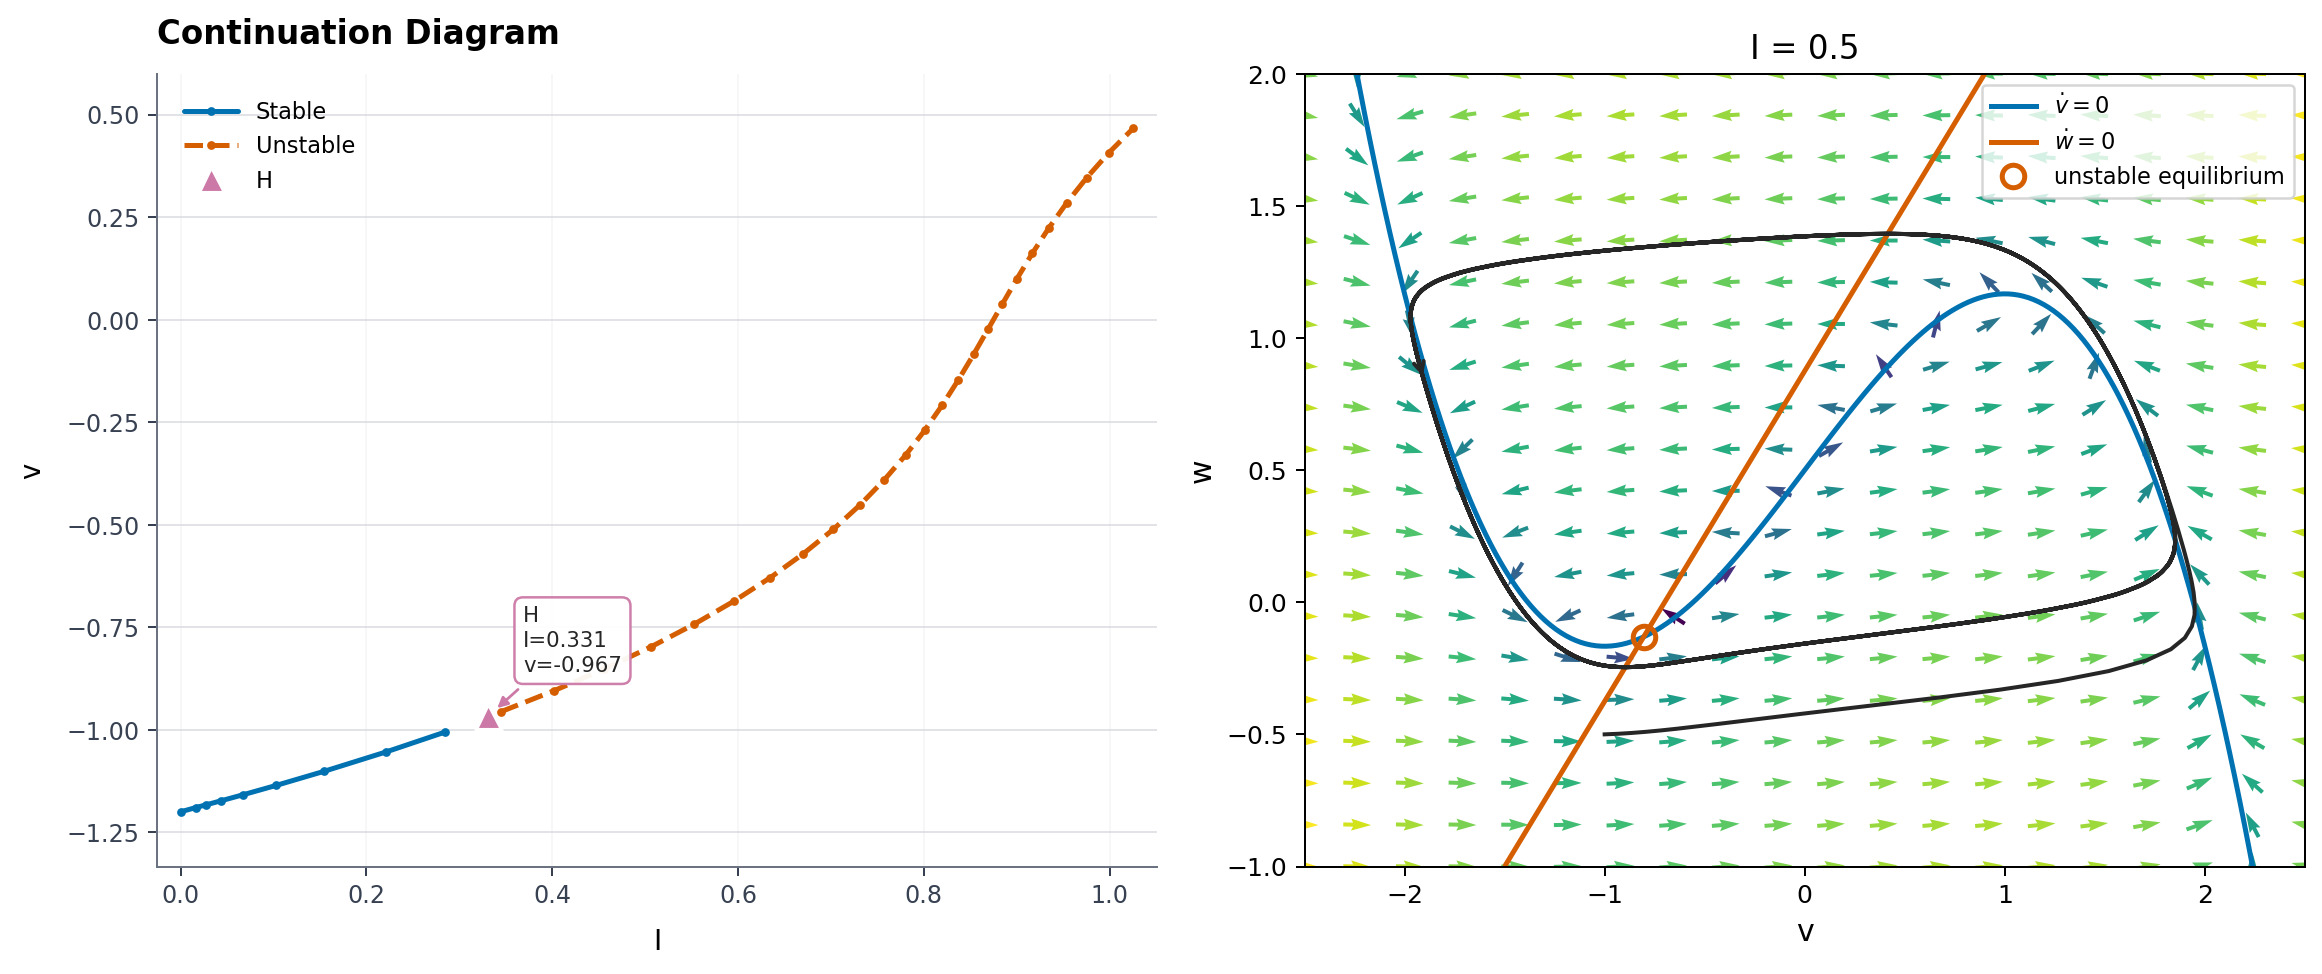
\includegraphics[width=.96\textwidth]{../../examples/images/example_12_fitzhugh_nagumo_phase_plane.jpg}
\vspace{-1mm}
\scriptsize
At $I\approx0.331$ the continued equilibrium changes stability. At $I=0.5$,
the hollow marker and outward trajectory provide a state-space interpretation;
they do not replace residual, spectrum, or event-refinement checks.
\end{frame}
